\documentclass[a4paper,english,titlepage,11pt]{article}

\usepackage{mathcomp,amssymb,verimagstudent}
\usepackage[utf8]{inputenc}
\usepackage[T1]{fontenc}
\usepackage{amsmath}
\usepackage{mathenv}
\usepackage{tikz}
\usepackage{listings}
\usepackage{placeins}
\usepackage{algorithm}
\usepackage{algpseudocode}

\newtheorem{definition}{Definition}[section]
\newtheorem{theorem}{Theorem}[section]
\newtheorem{proposition}[theorem]{Proposition}

\newcommand*\system[1]{\left[ \begin{array}{lllll}#1 \end{array}\right.}

\def\R{\mathbb{R}}
\def\Z{\mathbb{Z}}
\def\N{\mathbb{N}}
\def\Q{\mathbb{Q}}
\def\P{\mathcal{P}}
\def\ite{\textnormal{ite\ }}
\def\lfp{\textnormal{\it lfp}}

\definecolor{trefle}{rgb}{0,0.5,0}
\definecolor{moka}{rgb}{0.5,0.25,0}
\definecolor{minuit}{rgb}{0,0,0.5}

\tikzstyle{arrow}=[->,line width=.05cm,draw=red!90!blue!60!black]

\usetikzlibrary{snakes,arrows,shapes,backgrounds,shadows,automata,patterns}
\usepgflibrary{snakes}

\tikzstyle{state}=[circle,fill=black!25,minimum size=13pt,inner sep=0pt]
\tikzstyle{transition}=[rectangle,semithick,draw=black!75,
  			  minimum size=4mm]
\tikzstyle{transition2}=[transition,rectangle,thick,dashed,
  			  minimum size=4mm]
\tikzstyle{PRstate}=[circle,double,draw,fill=blue!15,minimum size=13pt,inner sep=0pt]
\tikzstyle{polyhedra}=[blue!25,opacity=0.5,pattern=north west lines,pattern
color=blue]
\tikzstyle{line}=[black,thick]

\lstnewenvironment{LLVM}
{\lstset{language=C,
		basicstyle=\ttfamily\footnotesize,
		commentstyle=\color{moka}\textit,
		keywordstyle=\color{minuit},
		identifierstyle=\color{trefle},
		showstringspaces=false}}
{}

\lstnewenvironment{C}
{\lstset{language=C,
		basicstyle=\ttfamily,
		commentstyle=\color{moka}\textit,
		keywordstyle=\color{minuit},
		identifierstyle=\color{trefle},
		showstringspaces=false}}
{}

\title{Static Analysis by Path Focusing}
\author{Julien Henry}
\date{2011}
\shorttitle{Static Analysis by Path Focusing}
\institute{Grenoble-INP}
\abstract{an abstract}
\keywords{keywords}
\tutor{David Monniaux - Matthieu Moy}
\notes{some notes}
\webaddress{Julien.Henry@imag.fr}
\reporttype{M2R internship's report}


\begin{document}
  
  \maketitlepage

  \tableofcontents
  
  \newpage


\section*{Introduction} 

Static analysis aims at automatically computing properties on programs, such as
the possible values of their variables during execution. This allows to show for
instance that a program will not overflow, will not divide by zero, to compute
loop invariants\dots
The main applications of static analysis are compilation-time optimisation, and
the proof of satefy properties in critical systems, such as avionics.

Abstract Interpretation is a general framework used for static analysis.
Linear Relation Analysis (LRA) is a direct application of this framework, that
computes an upper-approximation of the set of the possible states of a numerical
program. The state of a program is defined by the position of the program
counter in the code, and the current values of the different numerical variables.
The set of possible states is expressed as a least fixpoint of a set of
equations defining the semantics of the program. 

A fundamental fact in static analysis is that it cannot be perfectly precise:
either the set of possible states we compute is unsound (it doesn't contain all
the possible states during execution), or it is incomplete (it contains
states that can never be reached during execution). 
Abstract Interpretation is sound but incomplete, since it always computes an
upper-approximation of the set of possible states.

Linear Relation Analysis approximates the set of possible states as a convex
polyhedron where the dimensions are the numerical variables of the program.
Instead of convex polyhedra, one could choose intervals, octagons, etc.
The fixpoint equation is computed iteratively; that is, successive
approximations of the set of reachable states are computed until they converge
to a fixpoint. 

Satisfiability Modulo Theory (SMT) solving is a field in computer science that
aims to decide the satisfiability of a logic formula containing Boolean
predicates and elements of a theory, such as linear arithmetic relations between
integers.
In this report, we present a novel refinement of the Abstract Interpretation
technique, that uses SMT-solving to guide the fixpoint iterations, so that it
temporarily focuses on a selected path in the control flow graph (the graph
expressing the semantics of the program), in order to
obtain more precise results at reasonable cost.

\subsection*{Contribution and Organization}

In this report we make the following contributions:
\begin{itemize}
\item We present a new technique, refered as \emph{Path Focusing}, that takes
benefits of the recent advances in the field of SMT-solving to improve precision
of static analysis by abstract interpretation. We also present an adaptation of
this technique to compute disjunctive invariants.
\item We present an implementation of this technique into a small analyzer, as
well as the implementation of another technique proposed in \cite{GopanR06},
such as we can compare precision and cost of the these two methods.
\end{itemize}

The report is organized as follows:
Part \ref{stateoftheartpart} introduces the state of the art in Abstract
Interpretation and more specifically in Linear Relation Analysis.
Part \ref{pathfocusingpart} describes the two techniques
\emph{Lookahead Widening} and \emph{Path Focusing}.
Part \ref{implementationpart} presents the implementation of these two
techniques into an analyzer, and the experimental results we obtained.

\part{Abstract Interpretation: state of the art}
\label{stateoftheartpart}

\section{Introductive example}

We consider the following program:

\begin{figure}[!h]
   \begin{minipage}[c]{.46\linewidth}
\begin{C}
x = 0;
while (x < 100) {
	x++;
}
\end{C}
   \end{minipage} \hfill
   \begin{minipage}[c]{.46\linewidth}
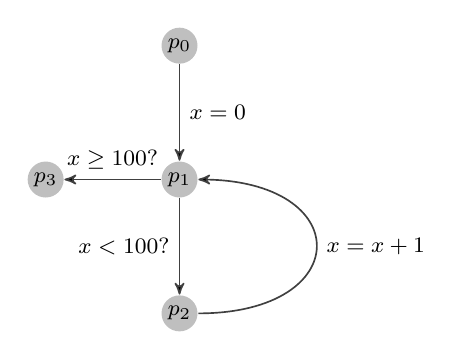
\begin{tikzpicture}[->,>=stealth',auto,node distance=1.7cm,
                    semithick,font=\footnotesize]

	\node[state] (n0) {$p_0$};
	\node[state] (n1) [below of=n0] {$p_1$};
	\node[state] (n2) [below of=n1] {$p_2$};
	\node[state] (n3) [left of=n1] {$p_3$};

  \path [transition] 
		(n0) edge              node {$x = 0$} (n1);
  \path [transition] 
        (n1) edge			   node [above] {$x \geq 100?$} (n3);
  \path [transition] 
        (n1) edge			   node [left] {$x < 100?$} (n2);
  \path [transition] 
        (n2) edge [out=0, in=0, distance=2cm] node [right] {$x = x+1$} (n1);

\end{tikzpicture}
   \end{minipage}
\end{figure}
\FloatBarrier

Static analysis aims to discover some properties about programs. In this
example, one would to compute the set of possible values for the variable $x$
during execution.
The graph at the right side represents the program. The nodes of the graph are
called \emph{program points}. We can compute for instance the set $Y_1$ of
values for $x$ at point $p_1$. This set depends on the sets $Y_0$ and $Y_2$,
since there are two edges arriving at $p_1$: the first one comes from $p_0$, and
the second one from $p_2$.

There is a relation between $Y_1$ and $Y_2$ :
\begin{eqnarray*}
Y_1 &=& \{x\ |\ x=0 \vee \exists x' \in Y_2, x=x'+1 \} \\
Y_2 &=& \{x\ |\ x \in Y_1 \wedge x < 100 \}
\end{eqnarray*}

We see that $Y_1$ and $Y_2$ can be computed step by step:
we start with $Y_1 = Y_2 = \emptyset$.
Then, we add iteratively new elements in the sets.
\begin{itemize}
\item  We see that $0 \in Y_1$: $Y_1 = \{0\}$.
\item $Y_1$ contains $0$. So, $Y_2$ also contains $0$ by definition: $Y_2 =
\{0\}$.
\item $Y_2$ contains $0$, so $0+1=1$ is in $Y_1$: $Y_1 = \{0,1\}$.
\item Again, we find $Y_2 = \{0,1\}$.
\item $Y_2$ now contains $1$, so $1+1=2 \in Y_1$: $Y_1 = \{0,1,2\}$.
\item We continue the iteration until we find no more elements in the sets\dots
\end{itemize}

This computation is a fixpoint computation: one updates the different sets until
we find no more elements. These sets are strictly increasing (we always add new
elements in the sets), and if we find no new elements to add, that means we have
reached a limit.

\section{Abstract Interpretation}

Abstract Interpretation \cite{CC77,CousotCousot92-1} is a general method to find approximate solutions of
fixpoint equations. This method is used for program analysis, since analyzing a
program often comes down to solving fixpoint equations $\Phi(x) = x$.

However, most of the time, the solution of this fixpoint equation must be
computed in a complex domain: in program analysis, this could be the state space
of the program, i.e the set of all possible states of the program. This
computation quickly becomes too costly or doesn't terminate.

\subsection{Abstraction of the domain}

Abstract Interpretation method proposes to represent more efficiently the
elements of this complex domain $C$ of concrete values, by choosing an simpler
domain  $A$ called \emph{abstract domain}. The relation between these two
domains is characterized by two functions, usually called 
$\alpha\ :\ C \mapsto A$, $\gamma \ : \ A \mapsto C$, such as:

$$\forall x \in C, \forall y \in A, \alpha(x) \leq_{A} y \Leftrightarrow x
\leq_{C} \gamma(y) $$

where $\leq_C$ and $\leq_A$ are the order relations on $C$ and $A$. Then, the
fixpoint computation is done in the abstract domain, using the approximation of
the function $\Phi$, i.e $\alpha(\Phi) = \alpha \circ \Phi \circ \gamma$, also
noted $\Phi^\#$.
We have the following result:

\begin{proposition}
If $C$ is a complete lattice, and if $\Phi$ is increasing from $C$ to $C$, then
$$\alpha(\lfp(\Phi)) \leq_A \lfp(\alpha(\Phi))$$
where $\lfp(\Phi)$ denotes the least fixpoint of $\Phi$.
\end{proposition}

In fact, one compute the least fixpoint of the function in the abstract
domain, and the result of the computation also gives an upper approximation of
the fixpoint in the concrete domain.


\subsection{Termination}

Termination of the fixpoint computation has to be guaranteed. This termination
depends on the properties of the abstract domain:
this one should be finite, or of finite depth, meaning that there doesn't exist
any sequence $(y_i)_{i \geq 0}$ of elements of the abstract domain $A$ such as
$\forall i \geq 0,\ y_i <_A y_{i+1}$. Indeed, in case of a domain of infinite
depth, the least fixpoint
computation could run indefinitely, since the ascending sequence of elements of
$A$ is infinite, and the fixpoint in never reached.


Most of the domains that are used for program analysis doesn't satisfy this
finiteness property. To ensure convergence in this case, another approximation
is performed: a new operator is defined, called \emph{widening operator}, that
extrapolates the limit of a sequence of abstract values
\cite{CC77,CousotCousot92-4}. This \emph{widening
operator} is usually noted $\nabla: A \times A \rightarrow A$, and satisfies
the following properties:

\begin{itemize}
\item $\forall y_1, y_2 \in A,\ y_1 \leq_A y_1 \nabla y_2$ and $y_2 \leq_A y_1
\nabla y_2$. This guarantees the correctness of the result.
\item For any increasing sequence $y_0 \leq_A y_1 \leq_A \dots$, the sequence
defined by 
$$\system{
y'_0 & = &  y_0 \\
y'_{i+1} & = &  y'_i\ \nabla\ y_{i+1},\ \  \forall i > 0
}$$
is not strictly increasing. Then, applying the widening operator when the
sequence may increase indefinitely makes the computation converge to a fixpoint
in finite time. 
\end{itemize}

\cite{Monniaux_HOSC09} gives a more general definition of the widening operator.

The least fixpoint of a function $\Phi^\#$ is noted $\overline{y}$ and is equal
to $\displaystyle \lim_{i \geq 0}\ y_i$, where $y_0 = \perp$ (the least element
of $A$) and $y_{i+1} = \Phi^\# (y_i)$. Instead of computing this least fixpoint,
one compute an upper approximation of it, by computing the following ascending
sequence:

$$\system{
y'_0 &=& \perp \\
y'_{i+1} &=& y'_i\ \nabla\ \Phi^\#(y'_i),\ \ \forall i > 0
}$$

which converges towards $\tilde{y}$, where $\tilde{y} \geq_A \overline{y}$.

$\tilde{y}$ is a correct upper approximation of the least fixpoint of $\Phi^\#$,
and the classical technique is to regain some precision lost by the widening
operator by computing a descending sequence:

$$\system{
y''_0 &=& \tilde{y} \\
y''_{i+1} &=& \Phi^\#(y''_i), \ \ \forall i > 0
}$$

Each element of this descending sequence is still an upper approximation of the
least fixpoint $\overline{y}$. So, this sequence often allows to find
approximate least fixpoints that are more precise than the one obtained after
the ascending sequence.

\section{Linear Relation Analysis}

Linear Relation Analysis \cite{CH78} (also noted LRA) is a direct application of
Abstract Interpretation. It aims at computing an upper approximation of the
reachable states of a program containing numerical variables. The set of
possible assignments for the numerical variables is abstracted by convex
polyhedron. This technique discovers invariant linear relations between
the numerical variables at each control point of a program.

This technique is:
\begin{itemize}
\item \emph{sound}: Each possible assignment for the variables in the real
program is included in the abstract value.
\item \emph{incomplete}: The abstract value also contains assignments for the
variables that are not possible in the real program.
\end{itemize}

\subsection{Convex polyhedra}

Let $x_1, x_2, \dots ,x_n$ be the numerical variables of a program (assume they
all are in $\Q$). A state of
the program is then a point $\overrightarrow{x} \in \Q^n$.

In $\Q^n$, the set of polyhedra ordered by inclusion is a lattice. The least element is $\perp$
(the empty polyhedron), and the greatest element is $\top$ (the whole $Q^n$).

The classical union of two convex polyhedra may not be a convex polyhedra.
Therefore, we use the convex hull operation, noted $\sqcup$, for joining
polyhedra. 
If $X_1, X_2$ are two convex polyhedra, $X_1 \sqcup X_2$ is the
smallest convex polyhedron containing both $X_1$ and $X_2$.

Since the domain of convex polyhedra is of infinite depth, a widening operator
is defined to ensure convergence of the technique. There have been various
work proposing a definition of the widening operator in LRA
\cite{CH78,Hal79,HPR97,BlanchetCousotEtAl_PLDI03}, in order to fight
against the loss of precision induced by widening.

\subsection{Program Analysis}

Throughout the report, a program will be represented by a control flow graph:
\begin{itemize}
\item $P$ is a finite set of control points.
\item $I_p$ is the (possibly empty)
set of initial values for each control point $p \in P$. For an initial control
point $p$, i.e a starting point of the program, $I_p$ is not empty. It is empty
in the other case.
\item $E \subseteq  P \times P$ is a set of directed edges. Each edge $e \in E$
has a semantic $\tau_e: \P(\Q^n) \rightarrow \P(\Q^n)$, $\P(\Q^n)$ being the set
of possible values of $\overrightarrow{x}$. $\tau_e$ maps a set of states before
the transition to the set of states after the transition.
\end{itemize}

\begin{figure}[!h]
   \begin{minipage}[c]{.46\linewidth}
\begin{C}
x = 0;
y = 0;
while (true) {
	if (x <= 50) 
		y++;
	else 
		y--;
	if (y < 0) break;
	x++;
}
\end{C}
   \end{minipage} \hfill
   \begin{minipage}[c]{.46\linewidth}
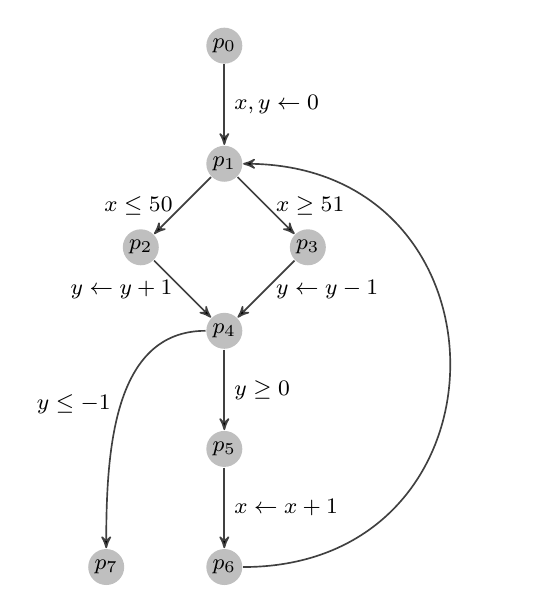
\begin{tikzpicture}[->,>=stealth',auto,node distance=1.5cm,
                    semithick,font=\footnotesize]

	\node[state] (n0) {$p_0$};
	\node[state] (n1) [below of=n0] {$p_1$};
	\node[state] (n2) [below left of=n1] {$p_2$};
	\node[state] (n3) [below right of=n1] {$p_3$};
	\node[state] (n4) [below left of=n3] {$p_4$};
	\node[state] (n5) [below of=n4] {$p_5$};
	\node[state] (n6) [below of=n5] {$p_6$};
	\node[state] (n7) [left of=n6] {$p_7$};

	\node (n8) [right of=n6] {};
	\node (n9) [right of=n1] {};

  \path [transition] 
		(n0) edge              node {$x,y \leftarrow 0$} (n1);
  \path [transition] 
        (n1) edge			   node [left] {$x \leq 50$} (n2);
  \path [transition] 
        (n1)  edge              node [right] {$x \geq 51$} (n3);
  \path [transition] 
        (n2) edge              node [left] {$y \leftarrow y+1$} (n4);
  \path [transition] 
        (n3) edge			   node [right] {$y \leftarrow y-1$} (n4);
  \path [transition] 
        (n4) edge			   node {$y \geq 0$} (n5);
  \path [transition] 
		(n4) edge  [out = 180, in=90] node [left] {$y \leq -1$} (n7);
  \path [transition] 
        (n5) edge              node {$x \leftarrow x+1$} (n6);
  \path [transition] 
        (n6) edge [out=0, in=0, distance=3.5cm] node {} (n1);

\end{tikzpicture}
   \end{minipage}
   \caption{Example of program, and its associate control flow graph. This
   program comes from \cite{GopanR06}.}
\label{runningexample}
\end{figure}
\FloatBarrier

To each state $p \in P$ of the control flow graph, we associate an abstract
value $X_p \in D$, $D$ being in our case the domain of convex polyhedra over
$\Q^n$. Since the exact operation $\tau$ may not be expressed in the abstract
domain, we abstract it into $\tau^\#$ such as $\forall X \in D, \tau(X)
\subseteq \tau^\#(X)$. 

The computation aims to find a solution for this system of abstract semantic
inequalities:

$$\system{
\forall p \in P, \ \ I_p \subseteq X_p \\
\forall (p',p) \in E,\ \  \tau^\#_{(p',p)}(X_{p'}) \subseteq X_p
}$$

\begin{figure}[h!]
\centering
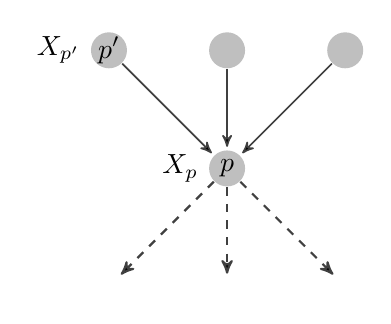
\begin{tikzpicture}[->,>=stealth',shorten >=1pt,auto,node distance=1.5cm,
                    semithick]

  \node[state] (p)             [label=left:$X_{p}$]       {$p$};
  \node[state]         (p2) [above  of=p] {};
  \node[state]         (p1) [left of=p2,label=left:$X_{p'}$] {$p'$};
  \node[state]         (p3) [right of=p2] {};
  \node         (p22) [below  of=p] {};
  \node         (p12) [left of=p22] {};
  \node         (p32) [right of=p22] {};

  \path [transition] (p1) edge              node {} (p);
  \path [transition] (p2) edge              node {} (p);
  \path [transition] (p3) edge              node {} (p);
  \path [transition2] (p) edge              node {} (p12);
  \path [transition2] (p) edge              node {} (p22);
  \path [transition2] (p) edge              node {} (p32);
\end{tikzpicture}
\end{figure}

The function $\Phi^\#$ previously described is the following:

$$\Phi^\#\left[ \begin{array}{c}
\vdots \\
X_p \\
\vdots
\end{array} \right] = \left[ \begin{array}{c} 
\vdots \\
I_p \sqcup \displaystyle \bigsqcup_{(p',p) \in E} \tau^\# (X_{p'}) \\
\vdots
\end{array} \right]$$

The fixpoint computation algorithm consist in replacing iteratively each $X_p$ by its value
on the right hand side, until the convergence.

In the case of an abstract domain with infinite ascending sequence, we use the
previously defined widening operator:

$$\left[ \begin{array}{c}
\vdots \\
X_p \\
\vdots
\end{array} \right] \longleftarrow \left[ \begin{array}{c} 
\vdots \\
X_p \nabla \left( I_p \sqcup \displaystyle \bigsqcup_{(p',p) \in E} \tau^\#
(X_{p'}) \right) \\
\vdots
\end{array} \right]$$


After a finite number of steps, the computation has reached the fixpoint and the
value $X_p$ at the end give the different linear relations between the
different numerical variables of the program at the control point $p$.

\subsection{Precision of the analysis}
In order to guarantee the termination of the computation, there is no need to
apply the widening operator at each control point $p \in P$. It is sufficient to
apply it on a subset of $P$, called $P_w$, such as removing the nodes of $P_w$
disconnects every cycles. For instance, one could choose $P_w$ as the set of the
heads of loops.

\subsubsection{Iteration strategies}
There exist several iteration strategies for computing the fixpoint: whatever
order we choose for updating the different $X_p, p\in P$, the result at the
end of the analysis is correct. Yet, the precision of the result and the time
before convergence could be very different. 
There have been some work to find efficient iteration strategies
\cite{Bou92}, such as first stabilizing innermost loops, or stabilizing strongly
connected components of the graph.

\subsubsection{Sources of imprecision}
 \label{multigraph}
Linear Relation Analysis is sound but incomplete: there is loss of precision
during the computation, due to various reasons:
\begin{enumerate}
\item Since an abstract domain is used to represent the set of possible states,
such as the domain of convex polyhedra, there is an upper approximation of the
set of possible states to the smallest convex polyhedra including this set. This
loss of precision is unavoidable. Still, there are techniques proposing to
compute disjunctive invariants \cite{GulwaniZ10} to limit this upper approximation: at each
program point, one compute a union of convex polyhedra instead of a single
one.
\item The widening operator, used to ensure convergence of the technique,
also induces a loss of precision. The classical technique is then to compute
narrowing iterations, which often recover some precision. 

For instance, considering the program:
\begin{C}
for (int i=0; i < 100; i++) {
}
\end{C}
The analysis starts with $i=0$. After one iteration, one obtain $i \in
[0,1]$, \dots. After a widening operation, the result becomes $i \in [0,
+\infty]$, which is an invariant, but very imprecise. We can do a new iteration,
with $i\in [0, +\infty]$ at the beginning of the loop, and we find that the
values for $i$ at the next step are in $[0, 100]$. This is still an invariant,
but much better.

\item There is also a loss of precision each time a point in the control flow
graph has several incoming edges. This is the case for instance for
\emph{if} statements, loops, etc. In this case, the abstract value of this point
is a convex hull of several convex polyhedra, inducing an upper approximation.
Indeed, if $X_1, X_2$ are convex polyhedra,
$$X_1 \cup X_2 \subseteq X_1 \sqcup X_2$$

To limit the number of such points, a method could be
to expand the control flow graph. For instance, instead of considering a graph
with a sequence of $n$ \emph{if-then-else} between point $p_1$ and $p_n$, one could remove the $n$ merge node
of these \emph{if-then-else}, each of them having two incoming edges, and adding 
$2^n$ edges from $p_1$ to $p_n$, corresponding to the different paths through
the \emph{if-then-else} statements. At the end, $p_n$ is the only point with
several incoming edges. This graph transformation results in an exponential
blowup, because of the exponential growth of the number of edges in the graph.
\end{enumerate}


\subsubsection{Acceleration}

Typically, to analyze a program with loops, the approach is to use the
widening operator, for example at the head of the loops, to ensure convergence.
Since this induces imprecision, another technique called \emph{acceleration}
aims to compute the exact effect of the loop when possible \cite{Gon07,GH06}. For instance, for
the following program, one could directly compute an invariant for the loop:


\begin{minipage}[c]{.39\linewidth}
\begin{C}
x = 0;
y = 0;
while (x < N) {
	y = y+2;
	x = x+5;
}
\end{C}
\end{minipage} 
\begin{minipage}[c]{.59\linewidth}
$$\begin{array}{llll}
\exists k \geq 0,& & x  = k \\
		&\wedge & y = 2k \\
		&\wedge & \forall k', (0 \leq k' \leq k)
				\Rightarrow (5k' \leq N)
\end{array}$$
\end{minipage}

Acceleration is possible when the loop is simple enough, and come to compute the
transitive closure $\tau_e^+$ of $\tau_e$, the transition function associated to
the loop.

\part{Path Focusing technique} \label{pathfocusingpart}
 
	In this part, we present two techniques that aim to isolate the different
	paths of the program to compute more precise invariants.

 \section{Lookahead Widening}

In some cases, a loop can have a non-regular behaviour, especially when it has
several paths. Some of these paths can stay impossible for a while, and become
possible after a certain number of iterations. However, the widening operator
extrapolates without taking care of these new possible paths. This can induce a
loss of precision, that Lookahead widening aims to limit.

Lookahead widening \cite{GopanR06} is a technique that aims to isolate the
different loop phases during the analysis, in order to obtain more precise
results.

In the program already depicted in figure \ref{runningexample}, there is a loop
with two perfectly distinct phases:
\begin{itemize}
\item During the 51 first iterations, both $x$ and $y$ are incremented.
\item During the 51 last iterations, $x$ is incremented and $y$ is decremented.
\end{itemize}

When computing the fixpoint iterations, we only consider a subset of the graph
for a while, until the convergence. In our example:
\begin{itemize}
\item Step 1:
	we only consider the path of
	the loop that is possible at the first iteration. The second path is
	ignored, and will be treated later. we compute the iterations, and we obtain
	an first invariant for this part of the graph. Then, we can do some
	narrowing steps in order to recover some precision, before adding new paths
	in the graph.
\item Step 2:
	Now, we add the new paths into our graph if they have become possible. In
	our case, the second path of the loop is now possible, so we add the path in
	the graph and compute new iterations until convergence\dots
\item Step 3: finally, the path from $p_4$ to $p_7$, so we add it into the graph and
compute the invariant for $p_7$.
\end{itemize}

\begin{figure}[!h]
   \begin{minipage}[c]{.46\linewidth}
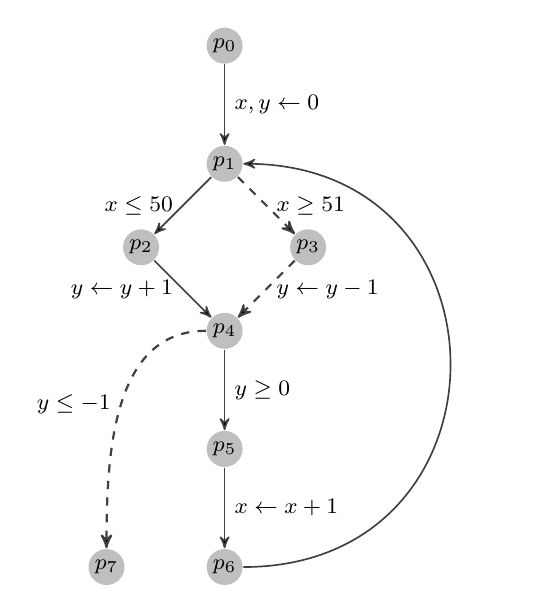
\begin{tikzpicture}[->,>=stealth',auto,node distance=1.5cm,
                    semithick,font=\footnotesize]

	\node[state] (n0) {$p_0$};
	\node[state] (n1) [below of=n0] {$p_1$};
	\node[state] (n2) [below left of=n1] {$p_2$};
	\node[state] (n3) [below right of=n1] {$p_3$};
	\node[state] (n4) [below left of=n3] {$p_4$};
	\node[state] (n5) [below of=n4] {$p_5$};
	\node[state] (n6) [below of=n5] {$p_6$};
	\node[state] (n7) [left of=n6] {$p_7$};

	\node (n8) [right of=n6] {};
	\node (n9) [right of=n1] {};

  \path [transition] 
		(n0) edge              node {$x,y \leftarrow 0$} (n1);
  \path [transition] 
        (n1) edge			   node [left] {$x \leq 50$} (n2);
  \path [transition2] 
        (n1)  edge              node [right] {$x \geq 51$} (n3);
  \path [transition] 
        (n2) edge              node [left] {$y \leftarrow y+1$} (n4);
  \path [transition2] 
        (n3) edge			   node [right] {$y \leftarrow y-1$} (n4);
  \path [transition] 
        (n4) edge			   node {$y \geq 0$} (n5);
  \path [transition2] 
		(n4) edge  [out = 180, in=90] node [left] {$y \leq -1$} (n7);
  \path [transition] 
        (n5) edge              node {$x \leftarrow x+1$} (n6);
  \path [transition] 
        (n6) edge [out=0, in=0, distance=3.5cm] node {} (n1);

\end{tikzpicture}
\centering Step 1
   \end{minipage} \hfill
   \begin{minipage}[c]{.46\linewidth}
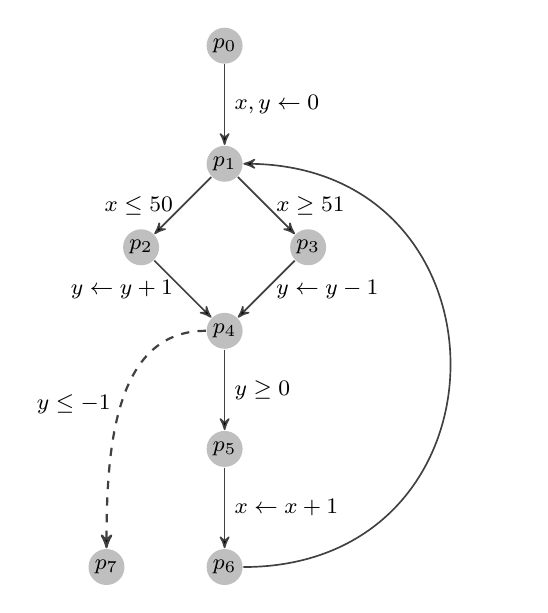
\begin{tikzpicture}[->,>=stealth',auto,node distance=1.5cm,
                    semithick,font=\footnotesize]

	\node[state] (n0) {$p_0$};
	\node[state] (n1) [below of=n0] {$p_1$};
	\node[state] (n2) [below left of=n1] {$p_2$};
	\node[state] (n3) [below right of=n1] {$p_3$};
	\node[state] (n4) [below left of=n3] {$p_4$};
	\node[state] (n5) [below of=n4] {$p_5$};
	\node[state] (n6) [below of=n5] {$p_6$};
	\node[state] (n7) [left of=n6] {$p_7$};

	\node (n8) [right of=n6] {};
	\node (n9) [right of=n1] {};

  \path [transition] 
		(n0) edge              node {$x,y \leftarrow 0$} (n1);
  \path [transition] 
        (n1) edge			   node [left] {$x \leq 50$} (n2);
  \path [transition] 
        (n1)  edge              node [right] {$x \geq 51$} (n3);
  \path [transition] 
        (n2) edge              node [left] {$y \leftarrow y+1$} (n4);
  \path [transition] 
        (n3) edge			   node [right] {$y \leftarrow y-1$} (n4);
  \path [transition] 
        (n4) edge			   node {$y \geq 0$} (n5);
  \path [transition2] 
		(n4) edge  [out = 180, in=90] node [left] {$y \leq -1$} (n7);
  \path [transition] 
        (n5) edge              node {$x \leftarrow x+1$} (n6);
  \path [transition] 
        (n6) edge [out=0, in=0, distance=3.5cm] node {} (n1);

\end{tikzpicture}
\centering Step 2
   \end{minipage}
   \caption{Dotted arrows are ignored by the analysis.}
\label{gopanreps}
\end{figure}
\FloatBarrier


 \section{Path Focusing}

	\subsection{Multigraph}

	\subsubsection{Expanding the control flow graph}
	The main idea of the technique is to compute the fixpoint iterations on an
	expanded multigraph instead of the classical control flow graph. A
	multigraph is a graph that can have several edges from a point $p$ to a
	point $q$. 

	Intuitively, expanding the graph comes back to consider independently the
	different paths in the control flow graph, and thus to be more precise,
	because paths that are not feasible will be ignored. Additionally, the
	number of control points with several incoming transitions will be reduced,
	so the loss of precision due to the convex hull of polyhedra may be
	minimized.

\begin{figure}[!h]
\label{multigraph}
\centering
\begin{minipage}[c]{.19\linewidth}
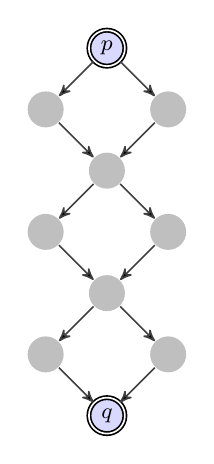
\begin{tikzpicture}[->,>=stealth',auto,node distance=1.1cm,
                    semithick,font=\footnotesize]

	\node[PRstate] (n0) {$p$};
	\node[state] (n1) [below left of=n0] {};
	\node[state] (n2) [below right of=n0] {};
	\node[state] (n3) [below right of=n1] {};
	\node[state] (n4) [below left of=n3] {};
	\node[state] (n5) [below right of=n3] {};
	\node[state] (n6) [below right of=n4] {};
	\node[state] (n7) [below left of=n6] {};
	\node[state] (n8) [below right of=n6] {};
	\node[PRstate] (n9) [below right of=n7] {$q$};

  \path [transition] 
		(n0) edge              node {} (n1);
  \path [transition] 
		(n0) edge              node {} (n2);
  \path [transition] 
		(n1) edge              node {} (n3);
  \path [transition] 
		(n2) edge              node {} (n3);
  \path [transition] 
		(n3) edge              node {} (n4);
  \path [transition] 
		(n3) edge              node {} (n5);
  \path [transition] 
		(n4) edge              node {} (n6);
  \path [transition] 
		(n5) edge              node {} (n6);
  \path [transition] 
		(n6) edge              node {} (n7);
  \path [transition] 
		(n6) edge              node {} (n8);
  \path [transition] 
		(n7) edge              node {} (n9);
  \path [transition] 
		(n8) edge              node {} (n9);
\end{tikzpicture}
\end{minipage} 
$\Longrightarrow$
\begin{minipage}[c]{.19\linewidth}
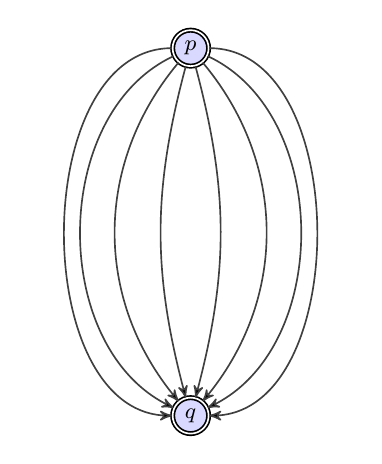
\begin{tikzpicture}[->,>=stealth',auto,node distance=1.1cm,
                    semithick,font=\footnotesize]

	\node[PRstate] (n0) {$p$};
	\node (n1) [below left of=n0] {};
	\node (n2) [below right of=n0] {};
	\node (n3) [below right of=n1] {};
	\node (n4) [below left of=n3] {};
	\node (n5) [below right of=n3] {};
	\node (n6) [below right of=n4] {};
	\node (n7) [below left of=n6] {};
	\node (n8) [below right of=n6] {};
	\node[PRstate] (n9) [below right of=n7] {$q$};

  \path [transition] 
		(n0) edge  [out=0, in=0]            node {} (n9);
  \path [transition] 
		(n0) edge  [out=180, in=180]        node {} (n9);
  \path [transition] 
		(n0) edge  [out=205, in=155]            node {} (n9);
  \path [transition] 
		(n0) edge  [out=230, in=130]            node {} (n9);
  \path [transition] 
		(n0) edge  [out=255, in=105]            node {} (n9);
  \path [transition] 
		(n0) edge  [out=-25, in=25]            node {} (n9);
  \path [transition] 
		(n0) edge  [out=-50, in=50]            node {} (n9);
  \path [transition] 
		(n0) edge  [out=-75, in=75]            node {} (n9);
\end{tikzpicture}
\end{minipage}
\caption{One can expand the graph in the left and obtain the associate graph in
the right.}
\end{figure}
\FloatBarrier

	Let $(P,E)$ be the control flow graph of the program.
	First, one choose a set of points $P_W \subseteq P$, such that the graph
	obtained after removing these points has no cycle. The widening operator
	will be applied at these points. The choice of $P_W$ can be guided by
	\cite{Bou92}.
	Then, one choose another set $P_R \subseteq P$ of nodes, satisfying the
	following properties:
	\begin{itemize}
	\item $I_p = \emptyset$ for each $p \in P \setminus P_R$, meaning that the initial
	points of the program are included in $P_R$.
	\item $P_W \subseteq P_R$: all the widening points are in $P_R$.
	\end{itemize} 

	The multigraph is then the graph such as:
	\begin{itemize}
	\item each element of $P_R$ is a point of the graph.
	\item for each path $p_1 \rightarrow p_2 \rightarrow \dots \rightarrow p_k$
	in the control flow graph, such as $p_1 \in P_R, p_k \in P_R$,
	there is a transition in the multigraph from $p_1$ to $p_k$ with the
	semantic $$\tau_{p_1 \rightarrow \dots \rightarrow p_k} = \tau_{p_{k-1}
	\rightarrow p_k} \circ
	\dots \circ \tau_{p_1 \rightarrow p_2}$$ where $\tau_{p_i \rightarrow
	p_{i+1}}$ is the transformation associated to the semantic of $p_i
	\rightarrow p_{i+1}$.
	\end{itemize}

	As explained in \ref{multigraph}, separating the different
	possible paths between $p$ and $q$ reduce the number of points with a join
	operation, and results in a better precision.
	This can result in an exponential blowup in the size of the graph. To avoid
	it, the technique is to never construct the multigraph, and only compute
	parts of it when needed.

	Intuitively, choosing a small set $P_R$ will result in a better precision,
	but a higher cost. 
	Indeed, the number of paths between two points of $P_R$ will grow if $P_R$
	contains few elements.
	A good choice for $P_R$ requires to find a good
	compromise between precision and cost of the technique.

\begin{figure}[!h]
\label{CFG}
\centering
\begin{minipage}[c]{.39\linewidth}
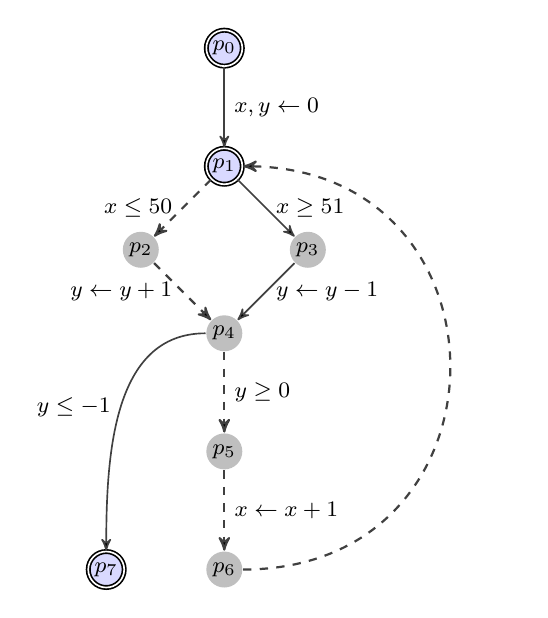
\begin{tikzpicture}[->,>=stealth',auto,node distance=1.5cm,
                    semithick,font=\footnotesize]

	\node[PRstate] (n0) {$p_0$};
	\node[PRstate] (n1) [below of=n0] {$p_1$};
	\node[state] (n2) [below left of=n1] {$p_2$};
	\node[state] (n3) [below right of=n1] {$p_3$};
	\node[state] (n4) [below left of=n3] {$p_4$};
	\node[state] (n5) [below of=n4] {$p_5$};
	\node[state] (n6) [below of=n5] {$p_6$};
	\node[PRstate] (n7) [left of=n6] {$p_7$};


  \path [transition] 
		(n0) edge              node {$x,y \leftarrow 0$} (n1);
  \path [transition2] 
        (n1) edge			   node [left] {$x \leq 50$} (n2);
  \path [transition] 
        (n1)  edge              node [right] {$x \geq 51$} (n3);
  \path [transition2] 
        (n2) edge              node [left] {$y \leftarrow y+1$} (n4);
  \path [transition] 
        (n3) edge			   node [right] {$y \leftarrow y-1$} (n4);
  \path [transition2] 
        (n4) edge			   node {$y \geq 0$} (n5);
  \path [transition] 
		(n4) edge  [out = 180, in=90] node [left] {$y \leq -1$} (n7);
  \path [transition2] 
        (n5) edge              node {$x \leftarrow x+1$} (n6);
  \path [transition2] 
        (n6) edge [out=0, in=0, distance=3.5cm] node {} (n1);
\end{tikzpicture}
\end{minipage} 
$\Longrightarrow$
\begin{minipage}[c]{.49\linewidth}
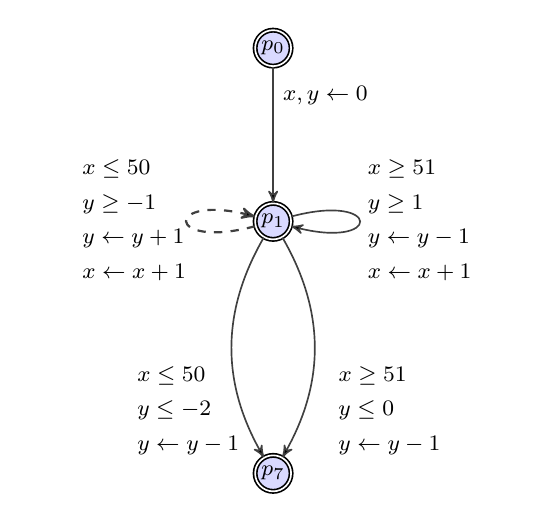
\begin{tikzpicture}[->,>=stealth',auto,node distance=3.2cm,
                    semithick,font=\footnotesize]

	\node[PRstate] (n0) {$p_0$};
	\node[PRstate] (n1) [below of=n0,yshift=1cm] {$p_1$};
	\node[PRstate] (n7) [below of=n1] {$p_7$};

	\node (n8) at (-3,0) {};
	\node (n8) at (3,0) {};

  \path [transition] 
		(n0) edge              node [yshift=5mm] {$x,y \leftarrow 0$} (n1);
  \path [transition] 
		(n1) edge    [bend left]  node [right,yshift=-0.8cm]  {$
		\begin{array}{l}
			x \geq 51 \\
			y \leq 0 \\
			y \leftarrow y-1
		\end{array}
		$} (n7);
  \path [transition2] 
		(n1) edge    [loop left,distance=1.2cm]  node [left,xshift=3mm] {$
		\begin{array}{l}
			x \leq 50 \\
			y \geq -1 \\
			y \leftarrow y+1 \\
			x \leftarrow x+1 
		\end{array}
		$} (n1);
  \path [transition] 
		(n1) edge    [loop right,distance=1.2cm]  node [right,xshift=-2mm] {$
		\begin{array}{l}
			x \geq 51 \\
			y \geq 1 \\
			y \leftarrow y-1 \\
			x \leftarrow x+1 
		\end{array}
		$} (n1);
  \path [transition] 
		(n1) edge    [bend right]  node [left,yshift=-0.8cm,xshift=4mm] {$
		\begin{array}{l}
			x \leq 50 \\
			y \leq -2 \\
			y \leftarrow y-1
		\end{array}
		$} (n7);
\end{tikzpicture}
\end{minipage}
\caption{Example of classical control flow graph, and its associate expanded
multigraph, where $P_R = \{p_0, p_1, p_7\}$. The path dashed from $p_1$ to $p_1$
in the control flow graph corresponds to a simple dashed transition in the multigraph,
having the same semantic.}
\end{figure}
\FloatBarrier

%\begin{tikzpicture}[->,>=stealth',auto,node distance=1.5cm,
%                    semithick,font=\footnotesize]
%
%	\node[state] (n0) {$p_0$};
%	\node[state] (n1) [below of=n0] {$p_1$};
%	\node[state] (n2) [below left of=n1] {$p_2$};
%	\node[state] (n3) [below right of=n1] {$p_3$};
%	\node[state] (n4) [below left of=n3] {$p_4$};
%	\node[state] (n5) [below of=n4] {$p_5$};
%	\node[state] (n6) [below of=n5] {$p_6$};
%	\node[state] (n7) [left of=n6] {$p_7$};
%
%	\node (n8) [right of=n6] {};
%	\node (n9) [right of=n1] {};
%	\node (n88) [above right of=n8] {};
%	\node (n99) [below right of=n9] {};
%
%	\path[transition] plot[->,smooth,tension=0.7] coordinates {
%		(n1)
%		(n2)
%		(-0.4,-3.8)
%		(n7)
%	};
%	\path[transition] plot[->,smooth,tension=0.7] coordinates {
%		(n1)
%		(0.7,-2.6)
%		(0,-3.8)
%		(n7)
%	};
%	\path[transition] plot[->,smooth,tension=0.7] coordinates {
%		(n1)
%		(-0.8,-2.4)
%		(-0.1,-3.8)
%		(0,-6.3)
%		(2.5,-5.5)
%		(2.5,-2.5)
%		(n1)
%	};
%	\path[transition] plot[->,smooth,tension=0.7] coordinates {
%		(n1)
%		(n3)
%		(0.3,-3.8)
%		(0.3,-6)
%		(2.1,-5.5)
%		(2.1,-2.5)
%		(n1)
%	};
%
%  \path [transition] 
%		(n0) edge              node {$x,y \leftarrow 0$} (n1);
%
%	\node[state] (n0) {$p_0$};
%	\node[state] (n1) [below of=n0] {$p_1$};
%	\node[state] (n2) [below left of=n1] {$p_2$};
%	\node[state] (n3) [below right of=n1] {$p_3$};
%	\node[state] (n4) [below left of=n3] {$p_4$};
%	\node[state] (n5) [below of=n4] {$p_5$};
%	\node[state] (n6) [below of=n5] {$p_6$};
%	\node[state] (n7) [left of=n6] {$p_7$};
%
%\end{tikzpicture}
	
	\subsubsection{Static Single Assignment form}

	Path focusing technique uses control flow graphs in static single assignment
	(SSA) form. The main concept behind the SSA form is that, syntactically,
	every variable is	
	only being assigned once. 


\begin{figure}[!h]
\centering
\begin{minipage}[c]{.39\linewidth}
\begin{C}
x = 0;
y = 0;
x = x + 2;
y = x + 1;
\end{C}
\end{minipage} 
$\Longrightarrow$ \hfill
\begin{minipage}[c]{.49\linewidth}
\begin{C}
x.0 = 0;
y.0 = 0;
x.1 = x.0 + 2;
y.1 = x.1 + 1;
\end{C}
\end{minipage}
\caption{On the left side, a simple program. On the right side, the same
program in SSA form.}
\end{figure}

This single definition property cannot be achieved with only the renaming of
variables assigned most than once. In some cases, two distinct definition reach
the same use, depending on the actual execution. To solve this issue, SSA form
uses $\Phi$-functions.

A $\Phi$-function is usually inserted at points of the control flow graph that
have several incoming transitions, and has the same number of arguments as the point
has incoming transitions. If we suppose these transitions are ordered, then the
$\Phi$-function returns the value of its $i$-th argument if the point is reached
from the $i$-th transition.

\begin{figure}[!h]
\centering
\begin{minipage}[c]{.39\linewidth}
\begin{C}
if (c) x = 0;
else x = 1;

y = x+1;
\end{C}
\end{minipage} 
$\Longrightarrow$ \hfill
\begin{minipage}[c]{.49\linewidth}
\begin{C}
if (c) x.0 = 0;
else x.1 = 0;

x.2 = Phi (x.0, x.1)
y.0 = x.2 + 1;
\end{C}
\end{minipage}
\end{figure}
\FloatBarrier

This static single assignment form is required for the computation of the focus
path.

	\subsection{Choice of the focus paths}

	\subsubsection{Reachability problem}
	\label{reachability}
	Path focusing technique aims to discover which paths to focus on for the
	computation of the fixpoint iterations. 
	Since the multigraph is not constructed explicitly, the different paths
	starting and finishing on node in $P_R$ are not known. 
	The technique proposes to express the focus path as the solution of a
	satisfiability modulo theory (SMT) problem:

	\begin{center} \emph{
		``Is there a path starting on control point $p$, with numerical
		variables in $X_p$, that ends on point $q$, with variables that are not
		in $X_q$ ?''}
	\end{center}

	This problem could be rephrased as:
	``Is there a path that starts on $p$, that can make the fixpoint computation
	progress ?''
	Indeed, the idea is to only focus on paths that make the abstract values
	grow.

	This is a reachability problem, that can be expressed as an SMT-formula,
	which is a logic formula with Boolean variables, and elements of a certain
	theory $T$. Depending on the program, one can choose different theories:
	\begin{itemize}
	\item For programs with rational variables, whose operations (instructions,
	transition conditions\dots) are all linear arithmetic, $T$ can be the theory
	of linear real arithmetic (LRA).
	\item For programs with integer variables (with a numerical state space in
	$\Z^n$) $T$ can be the theory of linear integer arithmetic (LIA).
	\end{itemize}

	Although deciding the satisfiability of such formula is NP-complete, there
	has been much research on decision procedures \cite{Kroening08} and there exist nowadays
	efficient programs, known as SMT-solvers, that can decide the satisfiability
	of LRA or LIA formulas. Well-known efficient SMT-solvers are
	Z3 \cite{MouraB08} and Yices \cite{DutertreM06}. 

	If the problem has a solution,  the SMT-solver will be in position to show
	which path in the control flow graph is selected, by giving a model: an
	assignments of the Boolean variables such that the formula is true.
	Among these Boolean variables, some of them are associated to a transition
	in the control flow graph:
	\begin{itemize}
	\item if the model has set to \emph{true} the Boolean variable $b_e$ associated
	to the transition $e$, then the focus path goes through this transition.
	\item in the other case, the focus path doesn't go through this transition.
	\end{itemize}
	
	Some others are associated to the points of the control flow graph. These
	are called \emph{reachability predicates}, and are set to \emph{true} in the
	model if and only if the focus path goes through these points.

	\subsubsection{Construction of the formula}
	The first point of the Path Focusing technique is to compute the SMT formula
	$\rho$ expressing the semantic of the program. For doing so, all the
	operations in the program have to be expressible within the theory we
	choose. Otherwise, the SMT-solver would not be able to decide if the formula
	is \emph{sat} or not.

	Since we want to find a path starting in a control point in $P_R$ and ending
	in a point in $P_R$, we need to disconnect in the formula the points $p_i$
	in $P_R$ into a source point $p_i^s$, with only outgoing transitions, and a
	destination point $p_i^d$, with only incoming transitions. 

	We construct the $\rho$ formula as follows:

\begin{enumerate}
\item Each numerical SSA variable of the control flow graph has its definition
in the $\rho$ formula.
\item For each operation in the program, we encode its semantic, expressed in
terms of the boolean and numerical SSA variables. For instance, if the CFG
contains the assignment $x.2 = x.1 + 1$, then we simply add $x.2 = x.1 + 1$ in
the formula. This equality expression is noted $assign(x.2)$. 
$assign(x)$ is defined for each numerical SSA-variable of the program.
\item For each transition $(p_i,p_j) \in E$, we set $t_{i,j} = B_i\ \wedge \
c(i,j)$, where $B_i = b_i^s$ if $p_i \in P_R$, or $b_i$ if not.
$c(i,j)$ express the condition that needs to be true to go through the
transition. For instance, $c(i,j)$ could be of the form $x < y$, \dots
If the transition is non-deterministic, then $c(i,j) = c_{i,j}$, where
$c_{i,j}$ is a boolean variable left non-deterministic.
\item For each point $p_i \notin P_R$, we set the reachability predicate 
$b_i = \displaystyle \bigvee_{(p_j,p_i)\in E} t_{j,i}$.
\item For each point $p_i^d \in P_R$, we set the reachability predicate 
$b_i^d = \displaystyle \bigvee_{(p_j,p_i)\in E} t_{j,i}$. 
\item Numerical $\Phi$-variables assignations have to be expressed in the $\rho$
formula. We simply use $\ite$ (\emph{if-then-else}) statements, standardly defined in the
SMT-Lib format \cite{BarST-SMTLIB}, for giving the right value to the variable,
depending on the incoming transition we come from. Generally, for a
$\Phi$-variable $x = \Phi(x_1,x_2,\dots,x_n)$ in control point $p_i$ with the
ordered incoming transitions $t_{j_1,i},t_{j_2,i},\dots,t_{j_n,i}$, we set:

$$x = \ite (t_{j_1,i})\  (x_1)\  (\ite (t_{j_2,i})\  (x_2)\  (\ite\  \dots))$$

where $\ite (c)\ (x)\ (y)$ is equal to $x$ if $c = true$, else $y$.

If the point where the $\Phi$-variable $x$ is defined is in
$P_R$, one need to rename $x$ into $x'$:
\begin{itemize}
\item $x$ will be the value of $x$ at the beginning of the path.
\item $x'$ will be the value of $x$ at the end of the path.
\end{itemize}
Indeed, there can be uses of $x$ along the path, and these uses refer to the
old value of $x$. 
\end{enumerate}

Finally, the $\rho$ formula is the following:

\begin{eqnarray*}
\rho = & \displaystyle\bigwedge_{p_i \notin P_R}& \left[ (b_i = \bigvee_{(p_h,p_i) \in E}
t_{h,i}) \wedge ( \bigwedge_{(p_i,p_j)\in E} t_{i,j} = b_i \wedge c(i,j))
\right] \wedge \\
 & \displaystyle\bigwedge_{p_i \in P_R}& \left[ (b_i^d = \bigvee_{(p_h,p_i) \in E}
 t_{h,i}) \wedge ( \bigwedge_{(p_i,p_j)\in E} t_{i,j} = b_i^s \wedge
 c(i,j)) \right] \wedge \\
 & \displaystyle\bigwedge_{x \in \Sigma}& assign(x)
\end{eqnarray*}

where $\Sigma$ is the set of the numerical SSA-variables of the program.

\begin{figure}[!h]
\begin{minipage}[c]{.49\linewidth}
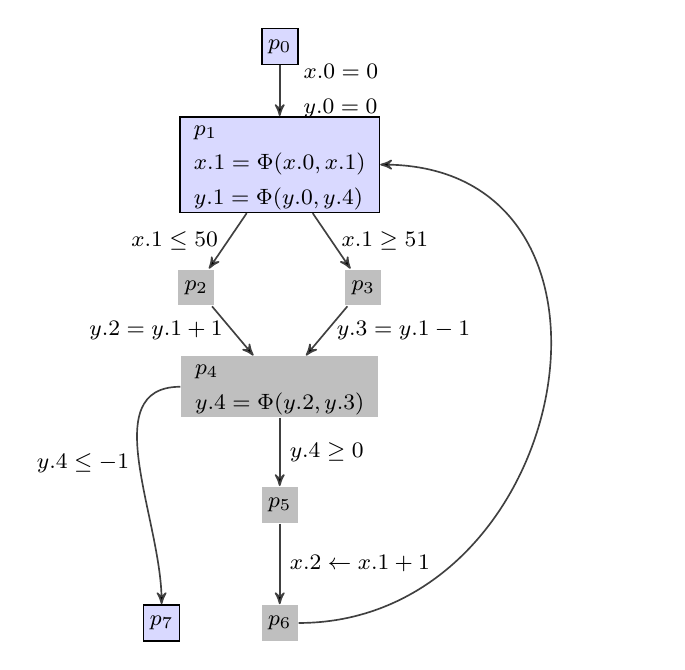
\begin{tikzpicture}[->,>=stealth',auto,node distance=1.5cm,
                    semithick,font=\footnotesize]

\tikzstyle{s}=[rectangle,fill=black!25,minimum size=13pt,inner sep=0pt]
\tikzstyle{t}=[rectangle,semithick,draw=black!75,
  			  minimum size=4mm]
\tikzstyle{PRs}=[rectangle,draw,fill=blue!15,minimum size=13pt,inner sep=0pt]
\tikzstyle{polyhedra}=[blue!25,opacity=0.5,pattern=north west lines,pattern
color=blue]
\tikzstyle{line}=[black,thick]

	\node[PRs] (n0) {$p_0$};
	\node[PRs] (n1) [below of=n0] {$\begin{array}{l}p_1 \\ x.1 =
	\Phi(x.0,x.1) \\ y.1 = \Phi(y.0,y.4)\end{array}$};
	\node[s] (n2) [below left of=n1,yshift=-0.5cm] {$p_2$};
	\node[s] (n3) [below right of=n1,yshift=-0.5cm] {$p_3$};
	\node[s] (n4) [below left of=n3,yshift=-0.2cm] {$\begin{array}{l}p_4\\ y.4 =
	\Phi(y.2,y.3)\end{array}$};
	\node[s] (n5) [below of=n4] {$p_5$};
	\node[s] (n6) [below of=n5] {$p_6$};
	\node[PRs] (n7) [left of=n6] {$p_7$};


  \path [transition] 
		(n0) edge              node {$\begin{array}{l} x.0 = 0 \\ y.0 =
		0\end{array}$} (n1);
  \path [transition] 
        (n1) edge			   node [left] {$x.1 \leq 50$} (n2);
  \path [transition] 
        (n1)  edge              node [right] {$x.1 \geq 51$} (n3);
  \path [transition] 
        (n2) edge              node [left] {$y.2 = y.1+1$} (n4);
  \path [transition] 
        (n3) edge			   node [right] {$y.3 = y.1-1$} (n4);
  \path [transition] 
        (n4) edge			   node {$y.4 \geq 0$} (n5);
  \path [transition] 
		(n4) edge  [out = 180, in=90] node [left] {$y.4 \leq -1$} (n7);
  \path [transition] 
        (n5) edge              node {$x.2 \leftarrow x.1+1$} (n6);
  \path [transition] 
        (n6) edge [out=0, in=0, distance=3.5cm] node {} (n1);
\end{tikzpicture}
(a) SSA form of the control flow graph seen in figure \ref{CFG}.
\end{minipage} 
$\Longrightarrow$ \hfill
\begin{minipage}[c]{.49\linewidth}
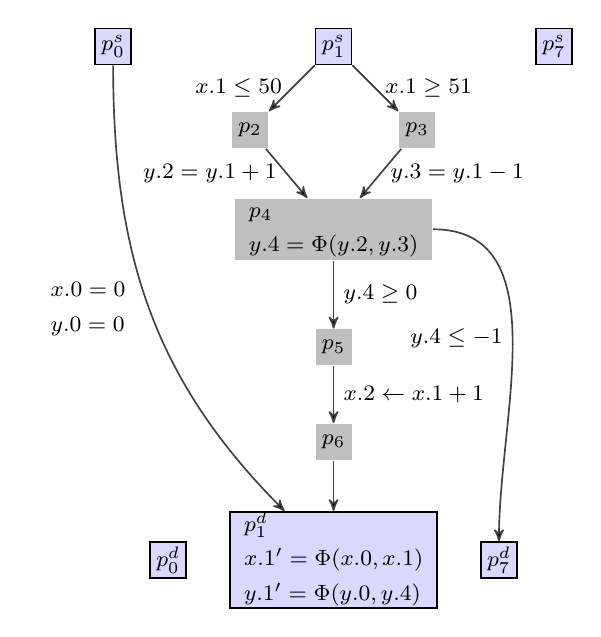
\begin{tikzpicture}[->,>=stealth',auto,node distance=1.5cm,
                    semithick,font=\footnotesize]

\tikzstyle{s}=[rectangle,fill=black!25,minimum size=13pt,inner sep=0pt]
\tikzstyle{t}=[rectangle,semithick,draw=black!75,
  			  minimum size=4mm]
\tikzstyle{PRs}=[rectangle,draw,fill=blue!15,minimum size=13pt,inner sep=0pt]
\tikzstyle{polyhedra}=[blue!25,opacity=0.5,pattern=north west lines,pattern
color=blue]
\tikzstyle{line}=[black,thick]

	\node[PRs] (n0s) {$p_0^s$};
	\node[PRs] (n1s) [right of=n0s,xshift=1.3cm] {$p_1^s$};
	\node[PRs] (n7s) [right of=n1s,xshift=1.3cm] {$p_7^s$};
	\node[s] (n2) [below left of=n1s] {$p_2$};
	\node[s] (n3) [below right of=n1s] {$p_3$};
	\node[s] (n4) [below left of=n3,yshift=-0.2cm] {$\begin{array}{l}p_4\\ y.4 =
	\Phi(y.2,y.3)\end{array}$};
	\node[s] (n5) [below of=n4] {$p_5$};
	\node[s] (n6) [below of=n5,yshift=0.3cm] {$p_6$};
	\node[PRs] (n1d) [below of=n6] {$\begin{array}{l}p_1^d \\ x.1' =
	\Phi(x.0,x.1) \\ y.1' = \Phi(y.0,y.4)\end{array}$};
	\node[PRs] (n7) [right of=n1d,xshift=0.6cm] {$p_7^d$};
	\node[PRs] (n0d) [left of=n1d,xshift=-0.6cm] {$p_0^d$};


  \path [transition] 
		(n0s) edge   [out=-90]           node [left] {$\begin{array}{l} x.0 = 0 \\ y.0 =
		0\end{array}$} (n1d);
  \path [transition] 
        (n1s) edge			   node [left] {$x.1 \leq 50$} (n2);
  \path [transition] 
        (n1s)  edge              node [right] {$x.1 \geq 51$} (n3);
  \path [transition] 
        (n2) edge              node [left] {$y.2 = y.1+1$} (n4);
  \path [transition] 
        (n3) edge			   node [right] {$y.3 = y.1-1$} (n4);
  \path [transition] 
        (n4) edge			   node {$y.4 \geq 0$} (n5);
  \path [transition] 
		(n4) edge  [out = 0, in=90] node [left] {$y.4 \leq -1$} (n7);
  \path [transition] 
        (n5) edge              node {$x.2 \leftarrow x.1+1$} (n6);
  \path [transition] 
        (n6) edge				node {} (n1d);
\end{tikzpicture}

(b) control flow graph (a), such as it is represented by the SMT formula $\rho$.
Points in $P_R$ have been split into a ``source'' point and a ``destination''
point, and $\Phi$-variables associated to points in $P_R$ have been primed.
\end{minipage} 
\caption{Example (cont'd)}
\end{figure}

	\subsubsection{Expression of the reachability problem}

	The SMT-formula $\rho$ express the semantic of the program. We still need to create the
	formula expressing the reachability problem defined in \ref{reachability}.

	The abstract domain $D$ we use is those of convex polyhedra, so an abstract
	value $X \in D$ is simply a system of linear inequalities between the
	different SSA-variables of the program. Then, it is easy to encode the
	property $x \in X$ into an SMT-formula: one simply writes the conjunction of
	these inequalities, with the name of the variables in the vector $x$.

	To compute the reachability strating from point $p_i$, the formula given to
	the SMT-solver is:

	$$\rho \wedge b_i^s \wedge \bigwedge_{j\neq i,\ j\in P_R} (\neg b_j^s)
	\wedge x_i \in X_{p_i} \wedge \bigvee_{j/(p_i,p_j)\in E} (b_2^d \wedge \neg
	(x_j' \in X_{p_j}))$$

	where $x_i$ is the vector of the SSA-variables at the beginning of the path,
	and $x_j'$ is the vector of the SSA-variable at the end: in this second
	vector, $\Phi$-variables defined in $p_j$ are primed.

	\begin{itemize}
	\item we search a path starting in $p_i$: $b_i^s$ has to be \emph{true}, and
	all other source points are \emph{false}.
	\item the vector $x_i$ of the numerical variables at point $p_i$ is in our
	abstract value $X_{p_i}$
	\item we search a path arriving in a successor $p_j$ of $p_i$, such as the
	vector of the numerical variables $x_j'$ is not yet included in the current
	abstract value $X_{p_j}$ of $p_j$. $b_j^d$ is \emph{true}, and the
	conjunction of the inequalities given by $X_{p_j}$ is \emph{false}.
	\end{itemize}

	\subsection{Algorithm}
	
	Path Focusing algorithm is described in Algorithm \ref{pathfocusingalgo}.
	We maintain a set $A$ of point in $P_R$ that need to be treated.
	We select iteratively one of these control points, and search for new focus
	paths starting from this point, until there is no more path to be treated.
	At the end of the analysis, one could perform some narrowing iterations in
	order to recover some precision.
\begin{algorithm}
\caption{Path Focusing}\label{pathfocusingalgo}
\begin{algorithmic}[1] 
\Procedure{pathfocusing}{$P$,$E$,$P_R$}
\ForAll {$p \in P_R$}
	\State Compute $Succ(p)$, the set of the successors of $p$ in the multigraph
\EndFor
\State $\rho \gets$ computeRho$(P,E)$
\State $A \gets \emptyset$
\ForAll {$p \in P_R / I_p \neq \emptyset$}
	\State $A \gets A \cup p$
\EndFor
\While{$A \neq \emptyset$}
	\State Select $p_i \in A$
	\State $A \gets A \setminus \{p_i\}$
	\While{true}
		\State $res \gets SmtSolve\left[\rho \wedge b_i^s \wedge
		\displaystyle\bigwedge_{\substack{j\neq i \\
		j\in P_R}} (\neg b_j^s) \wedge x_i \in X_{p_i} \wedge
		\bigvee_{\substack{j \\ p_j\in Succ(p_i)}} \left(b_2^d \wedge \neg (x'_j \in
		X_{p_j})\right)\right]$
		\If {$res = unsat$}
			\State \textbf{break}
		\EndIf
		\State Compute the focus path $e$ from $p_i$ to $p_j$
		\State $Y \gets \tau_e^\#(X_{p_i})$
		\If {$p_j \in P_W$}
			\State $X_{p_j} \gets X_{p_j} \nabla (X_{p_j} \sqcup Y)$
		\Else
			\State $X_{p_j} \gets X_{p_j} \sqcup Y$
		\EndIf
		\State $A \gets A \cup \{p_j\}$
	\EndWhile
\EndWhile
\State Possibly perform some narrowing steps
\State Compute $\{X_{p_i},\ i \notin P_R\}$
\State \textbf{return} $\{X_{p_i},\ i \in P\}$
\EndProcedure
\end{algorithmic}
\end{algorithm}

	\subsection {Precision of the analysis}

	One can refine the \emph{Path-focusing} algorithm by treating specially the
	self loops of the multigraph. Indeed, instead of simply apply the widening
	operator, one could compute some narrowing steps to regain precision before
	focusing on another path. This is the same principle as the one we find in
	\emph{Lookahead widening} \cite{GopanR06}.

	So, the algorithm has a special case if the path we focus on goes from $p_i$
	to itself: instead of computing $\tau_e^\#(X_{p_i})$, one compute
	$SelfLoop(\tau_e^\#,X_{p_i})$, defined in algorithm \ref{loopiteralgo}.

	The $SelfLoop$ procedure actually computes a widening operation, and
	computes a narrowing step in order to recover precision. In some cases,
	instead of performing widening/narrowing iterations, one could use
	acceleration techniques to find even more precise invariants \cite{GH06}.

	In order for this refinement to be precise, one needs to delay the widening
	operator when we consider a self-loop for the first time. Then, our
	algorithm uses a set $U$ of paths that have already been treated. If the
	self-loop we focus on is not in $U$, we apply a simple union instead of
	widening. Widening will be applied next time to guarantee the convergence.
	
\begin{algorithm}
\caption{SelfLoop}
\label{loopiteralgo}
\begin{algorithmic}[1] 
\Procedure{SelfLoop}{$\tau_e^\#$,$X_{p_i}$}
	\State $Y \gets \tau_e^\#(X_{p_i})$
	\State $X' \gets X_{p_i} \sqcup Y$
	\State $Y \gets \tau_e^\#(X')$
	\State \textbf{return} $Y$
\EndProcedure
\end{algorithmic}
\end{algorithm}

\begin{algorithm}
\caption{Path Focusing with special treatment for self loops}
\label{pathfocusingoptalgo}
\begin{algorithmic}[1] 
\Procedure{pathfocusing}{$P$,$E$,$P_R$}
\ForAll {$p \in P_R$}
	\State Compute $Succ(p)$, the set of the successors of $p$ in the multigraph
\EndFor
\State $\rho \gets$ computeRho$(P,E)$
\State $A \gets \emptyset$
\ForAll {$p \in P_R / I_p \neq \emptyset$}
	\State $A \gets A \cup p$
\EndFor
\While{$A \neq \emptyset$}
	\State Select $p_i \in A$
	\State $A \gets A \setminus \{p_i\}$
	\State $U \gets \emptyset$
	\While{true}
		\State $res \gets SmtSolve\left[\rho \wedge b_i^s \wedge
		\displaystyle\bigwedge_{\substack{j\neq i \\
		j\in P_R}} (\neg b_j^s) \wedge x_i \in X_{p_i} \wedge
		\bigvee_{\substack{j \\ p_j\in Succ(p_i)}} \left(b_2^d \wedge \neg (x'_j \in
		X_{p_j})\right)\right]$
		\If {$res = unsat$}
			\State \textbf{break}
		\EndIf
		\State Compute the focus path $e$ from $p_i$ to $p_j$
		\If{$p_i = p_j$}
			\State $Y \gets SelfLoop(\tau_e^\#,X_{p_i})$
		\Else
			\State $Y \gets \tau_e^\#(X_{p_i})$
		\EndIf
		\If {$(p_j \in P_W) \wedge (p_i \neq p_j \vee e \in U)$}
			\State $X_{p_j} \gets X_{p_j} \nabla (X_{p_j} \sqcup Y)$
		\Else
			\State $X_{p_j} \gets X_{p_j} \sqcup Y$
			\State $U \gets U \cup \{e\}$
		\EndIf
		\State $A \gets A \cup \{p_j\}$
	\EndWhile
\EndWhile
\State Possibly perform some narrowing steps
\State Compute $\{X_{p_i},\ i \notin P_R\}$
\State \textbf{return} $\{X_{p_i},\ i \in P\}$
\EndProcedure
\end{algorithmic}
\end{algorithm}

	\subsection{Disjunctive invariants}

	In this subsection, we propose an extension of the path focusing technique
	to compute disjunctive invariants, in order to improve precision of the
	analysis.

	\cite{GulwaniZ10} proposes a technique to compute transitive closure of a
	transition system, i.e compute the invariants for a loop having its semantic
	expressed by the transition system.

	A transition system for a control point $p$ is a DNF formula where each
	disjunct is the semantic of a path from $p$ to itself. It is of the form
	$$\bigvee_{1 \leq i \leq n} \tau_{p,i}$$ where $n$ is the number of
	paths, and $\tau_{p,i}$ is the semantic of the $i$-th path from $p$ to itself.

	The technique aims to compute a disjunctive invariant for this control
	point: 
	$$\displaystyle\bigvee_{1 \leq j \leq m} X_{p,j}$$
	where $X_{p,j}$ is a conjunction of linear inequalities, i.e a convex
	polyhedra.

	The essence of the method is to
	choose an integer $\delta \in \{1,..,m\}$, and a mapping function
	$\sigma: \{1,..,m\} \times \{1,..,n\} \mapsto \{1,..,m\}$.
	For each polyhedra of the disjunctive invariant, and for each path in the
	graph, the image of the polyhedra $X_{p,j}$ by the transition
	$\tau_{p,i}$ is joined with $X_{p,\sigma(j,i)}$.

\begin{algorithm}
\caption{Transitive closure}\label{gulwani}
\begin{algorithmic}[1] 
\Procedure{TransitiveClosure}{$\bigvee_{i=1}^n X_{p,i}$}
\ForAll {$j \in \{1,..,m\} \setminus \{\delta\}$}
	\State $X_{p,j} \gets \perp$
\EndFor
\State $X_{p,\delta} \gets Id$
\Repeat
	\For {$i \in \{1,..,n\}$ and $j \in \{1,..,m\}$}
		\State $X_{p,\sigma(j,i)} \gets X_{p,\sigma(j,i)} \sqcup
		\tau_{p,i}(X_{p,j})$
	\EndFor
\Until {no change in $\bigvee_{j=1}^m X_{p,j}$}
\EndProcedure
\end{algorithmic}
\end{algorithm}

There are heuristics to choose $m,\delta$ and $\sigma$ \cite[Section
5]{GulwaniZ10}.

This algorithm requires to enumerate all the paths and to compute their
semantics, which may result in an exponential blowup. In addition, the
\emph{for} loop at line $7$ iterates on all the $n \times m$ values of $(i,j)$:
some of the join operations may be useless, in the sense that the value of 
$X_{p,\sigma(j,i)}$ may not change. Here, one could use the same technique as
Path Focusing to avoid these drawbacks: one can use SMT-solving to find the
paths $\tau_{p,i}$.

\begin{algorithm}[!h]
\caption{Transitive closure with implicit transition system}\label{gulwani2}
\begin{algorithmic}[1] 
\Procedure{TransitiveClosureImplicit}{$p$}
\ForAll {$j \in \{1,..,m\} \setminus \{\delta\}$}
	\State $X_{j} \gets \perp$
\EndFor
\State $X_{\delta} \gets Id$
\While {true}

		\State $res \gets SmtSolve\left[\rho \wedge b_k^s \wedge
		\bigvee_{j=1}^m (B_j \wedge x \in X_{j})
		\wedge b_k^d
		\wedge \neg \left(\bigvee_{j=1}^m x' \in X_{j}\right)\right]$

	\If {$res = unsat$}
		\State \textbf{break}
	\EndIf
	\State Compute $\tau_{p,i}$ from $res$ 
	\State Take $j \in \{ k | B_k = true\}$ 
	\State $X_{p,\sigma(j,i)} \gets X_{p,\sigma(j,i)} \sqcup
	\tau_{p,i}(X_{p,j})$
\EndWhile
\EndProcedure
\end{algorithmic}
\end{algorithm}

The new algorithm we propose is described in Algorithm \ref{gulwani2}.
A difference is that here, we don't know the number of paths. Then, the mapping
function $\sigma$ has to be defined on $\{1,..,m\} \times \N$. We could also
compute this number of paths at the beginning of the algorithm.

\FloatBarrier
\part{Implementation}\label{implementationpart}

\emph{Lookahead Widening} and \emph{Path Focusing}
techniques have been implemented into a small analyzer, so that we can compare
the precision of their results. In this part, we explain some details about
these implementations.

 \section{Infrastructure}
The analyzer is based on the \emph{Low Level Virtual Machine} (LLVM)
\cite{LLVM:CGO04}, which is a compilation infrastructure used for instance by
the \emph{clang} compiler.

\subsection{LLVM internal representation}
% We need layers to draw the block diagram
\pgfdeclarelayer{background}
\pgfdeclarelayer{foreground}
\pgfsetlayers{background,main,foreground}

% Define a few styles and constants
\tikzstyle{sensor}=[draw, fill=blue!20, text width=5em, 
    text centered, minimum height=2.5em]
\tikzstyle{ann} = [above, text width=5em]
\tikzstyle{IR} = [sensor, text width=6em, fill=red!20, 
    minimum height=12em, rounded corners]
\def\leftdist{2.3}
\def\rightdist{5.0}
\def\edgedist{2.5}

\begin{figure}[!h]
\centering
\begin{tikzpicture}
    \node (IR) [IR] {\small Internal\\Representation\\ (IR)};
    % Note the use of \path instead of \node at ... below. 
    \path (IR.130)+(-\leftdist,0) node (c) [sensor] {C};
    %\path (IR.-150)+(-\leftdist,0) node (cpp) [sensor] {C++};
	\node [sensor] (cpp) [below of=c, yshift=-0.3cm] {C++};
	\node  (lang) [below of=cpp] {$\vdots$};
    
    \path (IR.130)+(+\rightdist,0) node (x8664) [sensor] {Binary\\ x86\_64};
	\node [sensor] (i686) [below of=x8664, yshift=-0.3cm] {Binary\\ i686};
	\node  (Out) [below of=i686] {$\vdots$};
	
	\path [draw, ->] (cpp) -- (IR);
	\path [draw, ->] (c) -- (IR);
	\path [draw, ->] (lang) -- (IR);

	\path [draw, ->] (IR) -- (x8664);
	\path [draw, ->] (IR) -- (i686);
	\path [draw, ->] (IR) -- (Out);
    
	% We could simply have written (gyros) .. (naveq.140). However, it's
    % best to avoid hard coding coordinates
    \node (Input) [below of=lang] {Input};
    \node (Output) [below of=Out] {Output};
    \path (IR.south west)+(-0.6,-0.4) node (Frontend) {Frontend};
    \path (IR.south east)+(+0.6,-0.4) node (Backend) {Backend};
    
    % Now it's time to draw the colored IMU and INS rectangles.
    % To draw them behind the blocks we use pgf layers. This way we  
    % can use the above block coordinates to place the backgrounds   
    \begin{pgfonlayer}{background}
        % Compute a few helper coordinates
        \path (c.west |- IR.north)+(-0.5,0.3) node (a) {};
        \path (Frontend.south -| x8664.east)+(+0.5,-0.2) node (b) {};
        \path[fill=yellow!20,rounded corners, draw=black!50, dashed]
            (a) rectangle (b);
        \path (c.north west)+(-0.2,0.2) node (a) {};
        \path (Input.south -| c.east)+(+0.2,-0.2) node (b) {};
        \path[fill=blue!10,rounded corners, draw=black!50, dashed]
            (a) rectangle (b);
        \path (x8664.north west)+(-0.2,0.2) node (a) {};
        \path (Output.south -| x8664.east)+(+0.2,-0.2) node (b) {};
        \path[fill=blue!10,rounded corners, draw=black!50, dashed]
            (a) rectangle (b);
    \end{pgfonlayer}
\end{tikzpicture}
\end{figure}
\FloatBarrier

The advantage of using such an infrastructure is that the analyzer can check
programs written in various languages: C, C++, \dots, without needing to write
a specific frontend for each of them. Here, the analyzer directly works on the
internal representation (IR), which is a graph representation of
the program. The control flow graph can easily be extracted from
this representation.

Our analyzer takes as parameter the LLVM internal representation of a program,
and returns linear relations between the numerical variables at each control
point of this program. It first applies some optimisation passes over the IR,
and then computes the linear relations by abstract interpretation.

\begin{figure}[!h]
\begin{minipage}[c]{.45\linewidth}
\begin{C}
int main() {
   int x = 0;
   int y = 0;

   while (1) {
      if (x <= 50) y++;
      else y--;

      if (y < 0) break;
      x++;
   }
}
\end{C}
\end{minipage}
\begin{minipage}[c]{.45\linewidth}
\includegraphics[width=8.5cm]{"images/cfg_gopan"}
\end{minipage}
\caption{Our running example and its internal representation in SSA form}
\end{figure}
\FloatBarrier

\subsection{Drawbacks}

During the implementation, we encountered problems due to the use of the LLVM
internal representation. Indeed, this format is not provided for static
analysis, but for code generation. Then, some informations we need for a precise
static analysis are lacking.

This is the case for the distinction between \emph{signed} and \emph{unsigned}
integers, which is inexistant in the representation, since the compiler doesn't
need this information to generate code. Yet, for static analysis, one need to
have this distinction to improve precision:
for instance, if $n$ is unsigned, one could add the constraint $n \geq 0$ in our
	abstract value at the beginning of the analysis.
	This lack of precision may be recovered by using disjunctive invariants: one
	could attach two polyhedra to the control point: the first one with the
	constraint $n \geq 0$, and the second one with $n < 0$.


Another example of information that was missing is the set of live variables.
Indeed, in LLVM, live variables computation is processed after the register
allocation. Then, the data structure we work on doesn't have live variables
informations yet. To solve this problem, we coded our own pass, that aims to
compute these live variables after the transformation in SSA form.

 \section{Abstract domain representation}

	The analyzer is implemented using the APRON library \cite{JM09}, which
	is a common interface to libraries implementing all the features
	for several abstract domains, such as convex polyhedra (NewPolka), 
	octagons (OCT), intervals (BOX).
	In our case, we used the convex polyhedra library, but we could switch
	to octagons or intervals easily.

	\subsection{Dimensions of the Abstract values}
	
	In our implementation, we tried to reduce as much as possible the dimensions
	of the abstract values at each program point. Indeed, there is no need to
	consider the whole set of the program numerical variables at each point $p$,
	since lots of these variables are not \emph{live} in $p$. 
	The definition of a \emph{live} variable is the following:

	\begin{definition}[Liveness]
	A variable is \emph{live} at the control point $p$ iff:
	\begin{itemize}
	\item its value is available at $p$, meaning that there is a path from the
	point defining the variable and $p$.
	\item its value might be used in the future, meaning that there exist a path
	starting in $p$, that arrives in a point using the variable.
	\end{itemize}
	\end{definition}

	LLVM internal representation allows to find the control point where
	a variable is defined and used, thanks to def-use chains: we can
	easily get the set of points where a variable is used, and we directly have
	a pointer to its definition.
	With all these informations, we implemented an LLVM pass that computes 
	the set of live variables in SSA, using the liveness check algorithm
	described in \cite[section 3.3]{Boi10}.

	
	At a program point $p$, the dimensions of the associate abstract value could
	only be the numerical variables that are live at $p$. This is
	not exactly the case in our implementation, because of another 
	optimisation: we only consider
	variables that are not a linear combination of other variables.

	For instance, assume that $x,y,z$ are numerical variables of a program,
	$x$ is defined as $x = y+z$, and $x,y,z$ are live at point $p$. Instead of having
	$x$ as a dimension for $X_p$, we only have $y$ and $z$. All the properties
	for $x$ can be directly extracted from $X_p$ and the information $x=y+z$.
	This is an optimisation in the sense that there is redundant information in
	the abstract value if both $x,y$ and $z$ are dimensions of $X_p$.

	Then, liveness definition can be adapted in our case:

	\begin{definition}[Liveness\dots]
	A variable $v$ is \emph{live\dots} at the control point $p$ iff:
	\begin{itemize}
	\item 
	its value is available at $p$, meaning that there is a path from the
	point defining the variable to $p$,
	\item one of these conditions holds:
		\begin{itemize}
		\item $v$ is live in $p$.
		\item There is a variable $v'$, defined as a linear combination of other
		variables $v_1, v_2, \dots, v_n$, such that $\exists i \in \{1,\dots,n\}, v = v_i$,
		and $v'$ is live\dots in $p$.
		\end{itemize}
	\end{itemize}
	\end{definition}

	Finally, a variable is a dimension of $X_p$ iff it is live\dots and it is
	not defined as a linear combination of program variables.

	\subsection{SMT-solving}

	\emph{Path focusing} technique requires to decide the satisfiability of some
	SMT formula, and to extract a model when the formula is satisfiable, i.e an
	assignement of the variables such that the formula is \emph{true}. For doing
	this, our implementation has an interface with Microsoft Z3 \cite{MouraB08},
	and Yices \cite{DutertreM06}. One can easily switch from one to another with
	an argument we give as parameter to the analyzer. In this way, we can
	compare the effectiveness of both SMT-solvers.


 \section{Experiments}

	To Be Completed


  \section*{Conclusion}
  
	To Be Completed

  \appendix
  

\bibliographystyle{plain}
  \bibliography{report}
\end{document}
